\documentclass[preprint2]{aastex62}

\bibliographystyle{aasjournal}

\usepackage{graphicx}
\usepackage[suffix=]{epstopdf}
\usepackage{natbib}
\usepackage{amsmath}
\usepackage{url}
\usepackage{xspace}

%    Make Scientific Notation
\providecommand{\e}[1]{\ensuremath{\times 10^{#1}}}

% make the word Kepler italicized
\newcommand{\Kepler}{\textsl{Kepler}\xspace}



\begin{document}
%%%%%%%%%%%%%%%%%%%%%%
\title{Rotating Stars from \Kepler Observed with Gaia DR2}

\shorttitle{Rotating Stars from \Kepler Observed with Gaia DR2}
\shortauthors{Davenport \& Covey}


\correspondingauthor{James. R. A. Davenport}
\email{James.Davenport@wwu.edu}

\author{James. R. A. Davenport}
\altaffiliation{NSF Astronomy and Astrophysics Postdoctoral Fellow}
\altaffiliation{DIRAC Fellow}
\affiliation{Department of Physics \& Astronomy, Western Washington University, 516 High St., Bellingham, WA 98225, USA}
\affiliation{Department of Astronomy, University of Washington, Seattle, WA 98195, USA}


\author{Kevin R. Covey}
\affiliation{Department of Physics \& Astronomy, Western Washington University, 516 High St., Bellingham, WA 98225, USA}


 
 

%%%%%%%%%%%%%%%%%%%%%%%%%%%%%%
\begin{abstract}
We have matched the astrometric data from {\em Gaia} Data Release 2 to the sample of stars with measured rotation periods from \Kepler. Using 30,305 stars with good distance estimates, we select 16,248 as being likely main sequence single stars centered within a 0.5 mag region about a 1 Gyr isochrone, removing many sub-giants and unresolved binary stars from the sample.
The rotation period bimodality, originally discovered by \citet{mcquillan2013}, is recovered for stars out to 525pc, but is not detectable at further distances. This bimodality correlates with Galactic height as well, dropping strongly for stars above $Z>90$ pc
We also find a significant width in the stellar main sequence of $M_G\sim$0.25 mag, as well as an increase in the average rotation period correlated with the $M_G$ offset at a given color (mass). We interpret this to be the measurable change in luminosity and loss of angular momentum as stars evolve along the main sequence, which may provide a new independent test of both stellar evolution and gyrochronlogy models.
%This investigation represents the first step in understanding the star formation history of our solar neighborhood as traced through stellar angular momentum loss. 
\end{abstract}



%%%%%%%%%%%%%%%%%%%%%%%%%%%%%%
\section{Introduction}

The \Kepler mission \citep{borucki2010}, through its unmatched combination of photometric precision and years-long observation baseline, has produced the largest sample of rotating stars to date. Stellar rotation has long been noted as a means to possibly age-date stars due to their constant angular momentum loss via winds
\citep{skumanich1972}. While studies of open clusters give hope that this ``gyrochronology'' model broadly works for solar-type and lower-mass stars, many uncertainties exist about the details of this spin-down and its utility as a clock. These include questions about the initial rotation period distribution for stars \citep[e.g.][]{barnes2010,matt2015}, the specific analytic prescription for modeling the spin-down \citep{angus2015}, and exploring the efficiency of this angular momentum loss mechanism at older ages \citep{van-saders2016}.


One of the most compelling results from the rotating star sample in \Kepler is the discovery of a bimodal period distribution.
\citet{mcquillan2013} first found a bimodality in the distribution of field M dwarfs with periods between $\sim$10 and $\sim$50 days. This feature was also found in the \Kepler field K dwarfs in \citep{mcquillan2014}. Using Gaia DR1, \citet{davenport2017} was able to remove contaminating sub-giants from the rotation sample and found the bimodality extended to the G dwarfs as well. This bimodal rotation period distribution is either a new short-lived transition or instability phase of angular momentum loss, or a signature of star formation history imprinted in the present-day rotation period distribution. However, to date this feature has only been observed in the \Kepler rotation period catalog, and most critically only for stars within $\sim$300 pc.



In this paper we follow the work of \citet{davenport2017} in refining the \Kepler rotation period sample using astrometric data from the {\em Gaia} mission \citep{gaia}. By matching the \citet{mcquillan2014} rotation period catalog to the newest data from {\em Gaia} Data Release 2 \citep{gaia_dr2}, we can use precise distances for essentially every star to select the most-likely main sequence dwarfs to distances well over 1 kpc. Importantly this filters out both sub-giants, the main contaminant noted by \cite{davenport2017}, and unresolved binary stars.
Here we demonstrate the power of such a combined time-domain and astrometric sample for constraining the detailed evolution of main sequence stars themselves, and exploring the star formation history of the Milky Way.
 



%%%%%%%%%%%%%%%%%%%%%%
\section{The \Kepler--Gaia Data}

We used the largest homogeneous catalog of rotation periods available from the \Kepler mission. The sample from \citet{mcquillan2014} provides rotation periods for more 34,030 stars, measured using the Auto-Correlation Function (ACF). While the ACF does not have as fine of resolution in recovering periods as compared with methods such as the Lomb-Scargle Periodogram, it is more robust to detecting the true period as opposed to an alias, and more complete for batch analysis of all stars \citep[e.g. see][]{aigrain2015}.

The \Kepler data was matched to the {\em Gaia} DR2 source catalog using a 1 arcsecond radius. We used the \Kepler--Gaia cross-match made publicly available by M. Bedell, which included entries for 195,830 sources. \Kepler-based stellar parameters included in this cross-match come the Data Release 25 \Kepler catalog. Joining this cross-matched table to the \citet{mcquillan2014} catalog, we found 33,538 sources.

To select stars with good parallaxes, as well as high quality photometry from {\em Gaia}, we selected stars with the following criteria:
\begin{itemize}
\item Parallax error $< 0.1$ mas
\item $\sigma(M_{G}) / M_{G} < 0.01$
\item $\sigma(G_{BP}) /G_{BP} < 0.01$
\item $\sigma(G_{RP}) /G_{RP} < 0.01$
\end{itemize}

Rather than simply use the inverse {\em Gaia} parallax values to measure the distance to sources, we use the improved distance prescription from \citet{bailer-jones2018}, who provided independent distances estimates for 1.33 billion {\em Gaia} sources using a weak prior on the distribution of stars in our galaxy. We follow their suggested use of the distance catalog, we only include sources with {\tt modality\_flag} == 1 (i.e. not a bimodal distance solution) and {\tt result\_flag} == 1 (i.e. a well constrained distance).
              

Our final sample contained 30,305 stars in {\em Gaia} DR2 with measured \Kepler rotation periods that passed these selection criteria. A color--magnitude diagram (CMD) of this sample using the {\em Gaia} bands is presented in Figure \ref{fig:cmd}, with points colored by their measured \Kepler rotation periods.


\begin{figure}[]
\centering
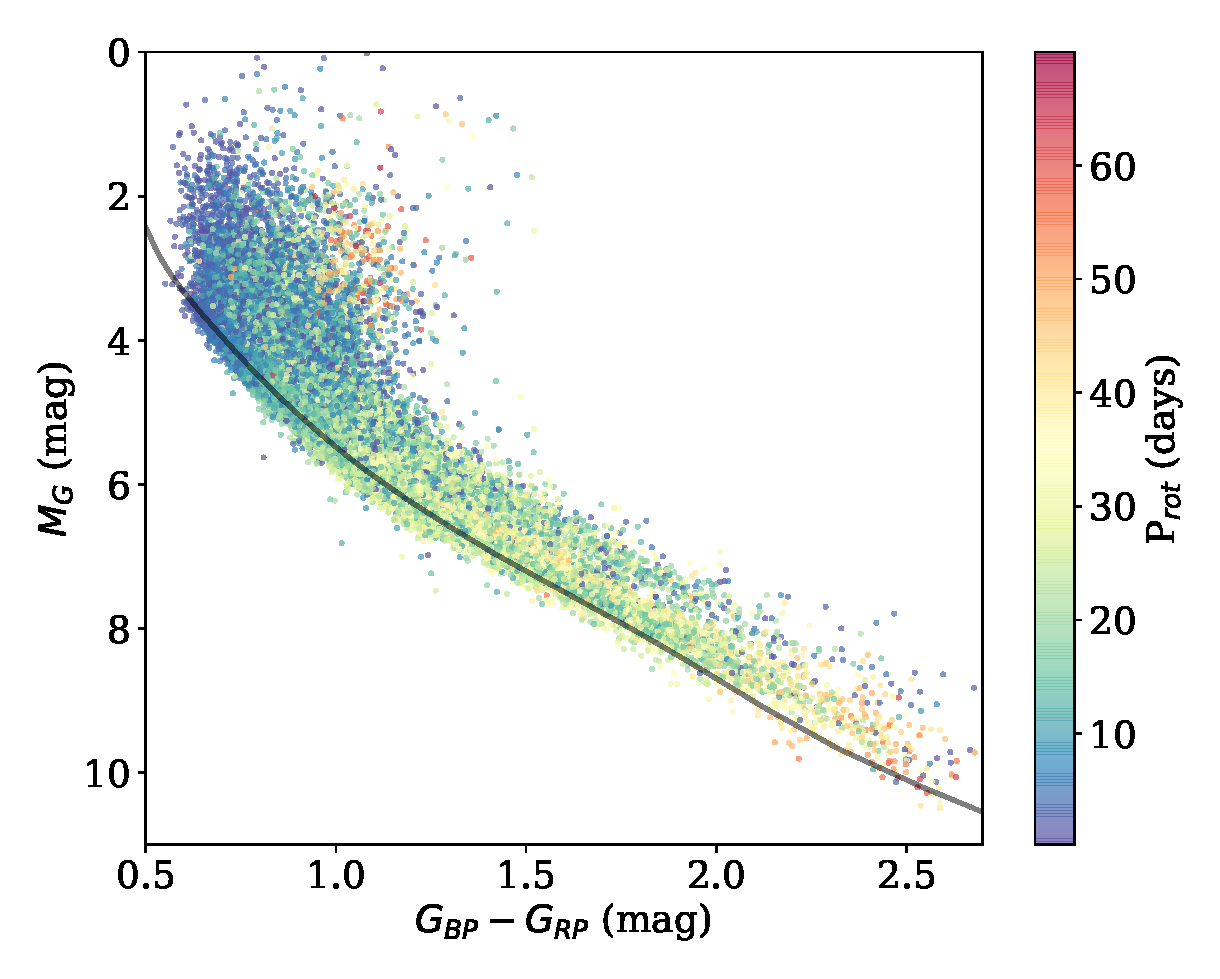
\includegraphics[width=3.6in]{../figures/cmd}
\caption{
Color--magnitude diagram for 30,305 \Kepler stars from the \citet{mcquillan2014} sample that are included in {\em Gaia} DR2, colored by their measured rotation period. For reference we show a $10^9$ year MIST isochrone (black line) used to select likely main sequence, single stars (black line). A track of binary stars is apparent $\sim$0.75 mag above the main sequence. As in \citet{davenport2017}, we find significant contamination of the rotation period sample for bluer stars by sub-giants.}
\label{fig:cmd}
\end{figure}




%%%%%%%%%%%%%%%%%%%%%%
\section{Selecting Main Sequence Stars}

As in \citet{davenport2017}, the color--magnitude diagram in Figure \ref{fig:cmd} shows many of the bluer stars in the \citet{mcquillan2014} sample are located significantly above the main sequence. These are likely subgiant stars, which do not follow the main sequence stars spin-down evolution \citep[e.g.][]{donascimento2012, van-saders2013}. Since \citet{davenport2017} found subgiants could obscure the rotation period bimodality for G dwarfs, these must be excluded from our analysis, but we encourage future studies to explore the wealth of angular momentum evolution data from these most-main sequence objects.

Beyond the subgiant contamination, we also see a secondary population of stars in a parallel track $\sim$0.75 mag above the normal main sequence, which are attributed to unresolved binary star systems. This pile-up above the main sequence occurs due to unresolved equal-mass (or nearly equal-mass) field binaries, and was seen in the {\em Gaia} DR1 data as well \citep{anderson2017}. Since these systems may have experienced tidal evolution that could significantly impact their rotation evolution \citep[e.g.][]{lurie2017}, we must also remove these from our analysis. Though we do not explore the binary population in any detail here, this sample (perhaps with radial velocity follow-up) may provide useful insight into the tidal evolution of binary stars, and are good targets for characterizing binary star system properties. We also note a small number of systems above the even the equal-mass binary main sequence track, which could be due to unresolved triple star systems.

We use an isochrone from the Mesa Isochrones and Stellar Tracks suite \citep[MIST;][]{MIST} to choose likely main sequence stars in Figure \ref{fig:cmd}. Our favored model to represent the main sequence in this study had [Fe/H] = +0.25 and an age of $10^9$ years, and was chosen by-hand. Single, main sequence stars were selected in a region spanning 0.1 mag fainter and 0.4 mag brighter than the MIST isochrone, resulting in a final sample  of 16,248 stars for analysis of their rotation period distributions.







%%%%%%%%%%%%%%%%%%%%%%
\section{Tracing the Period Bimodality}

\begin{figure*}[]
\centering
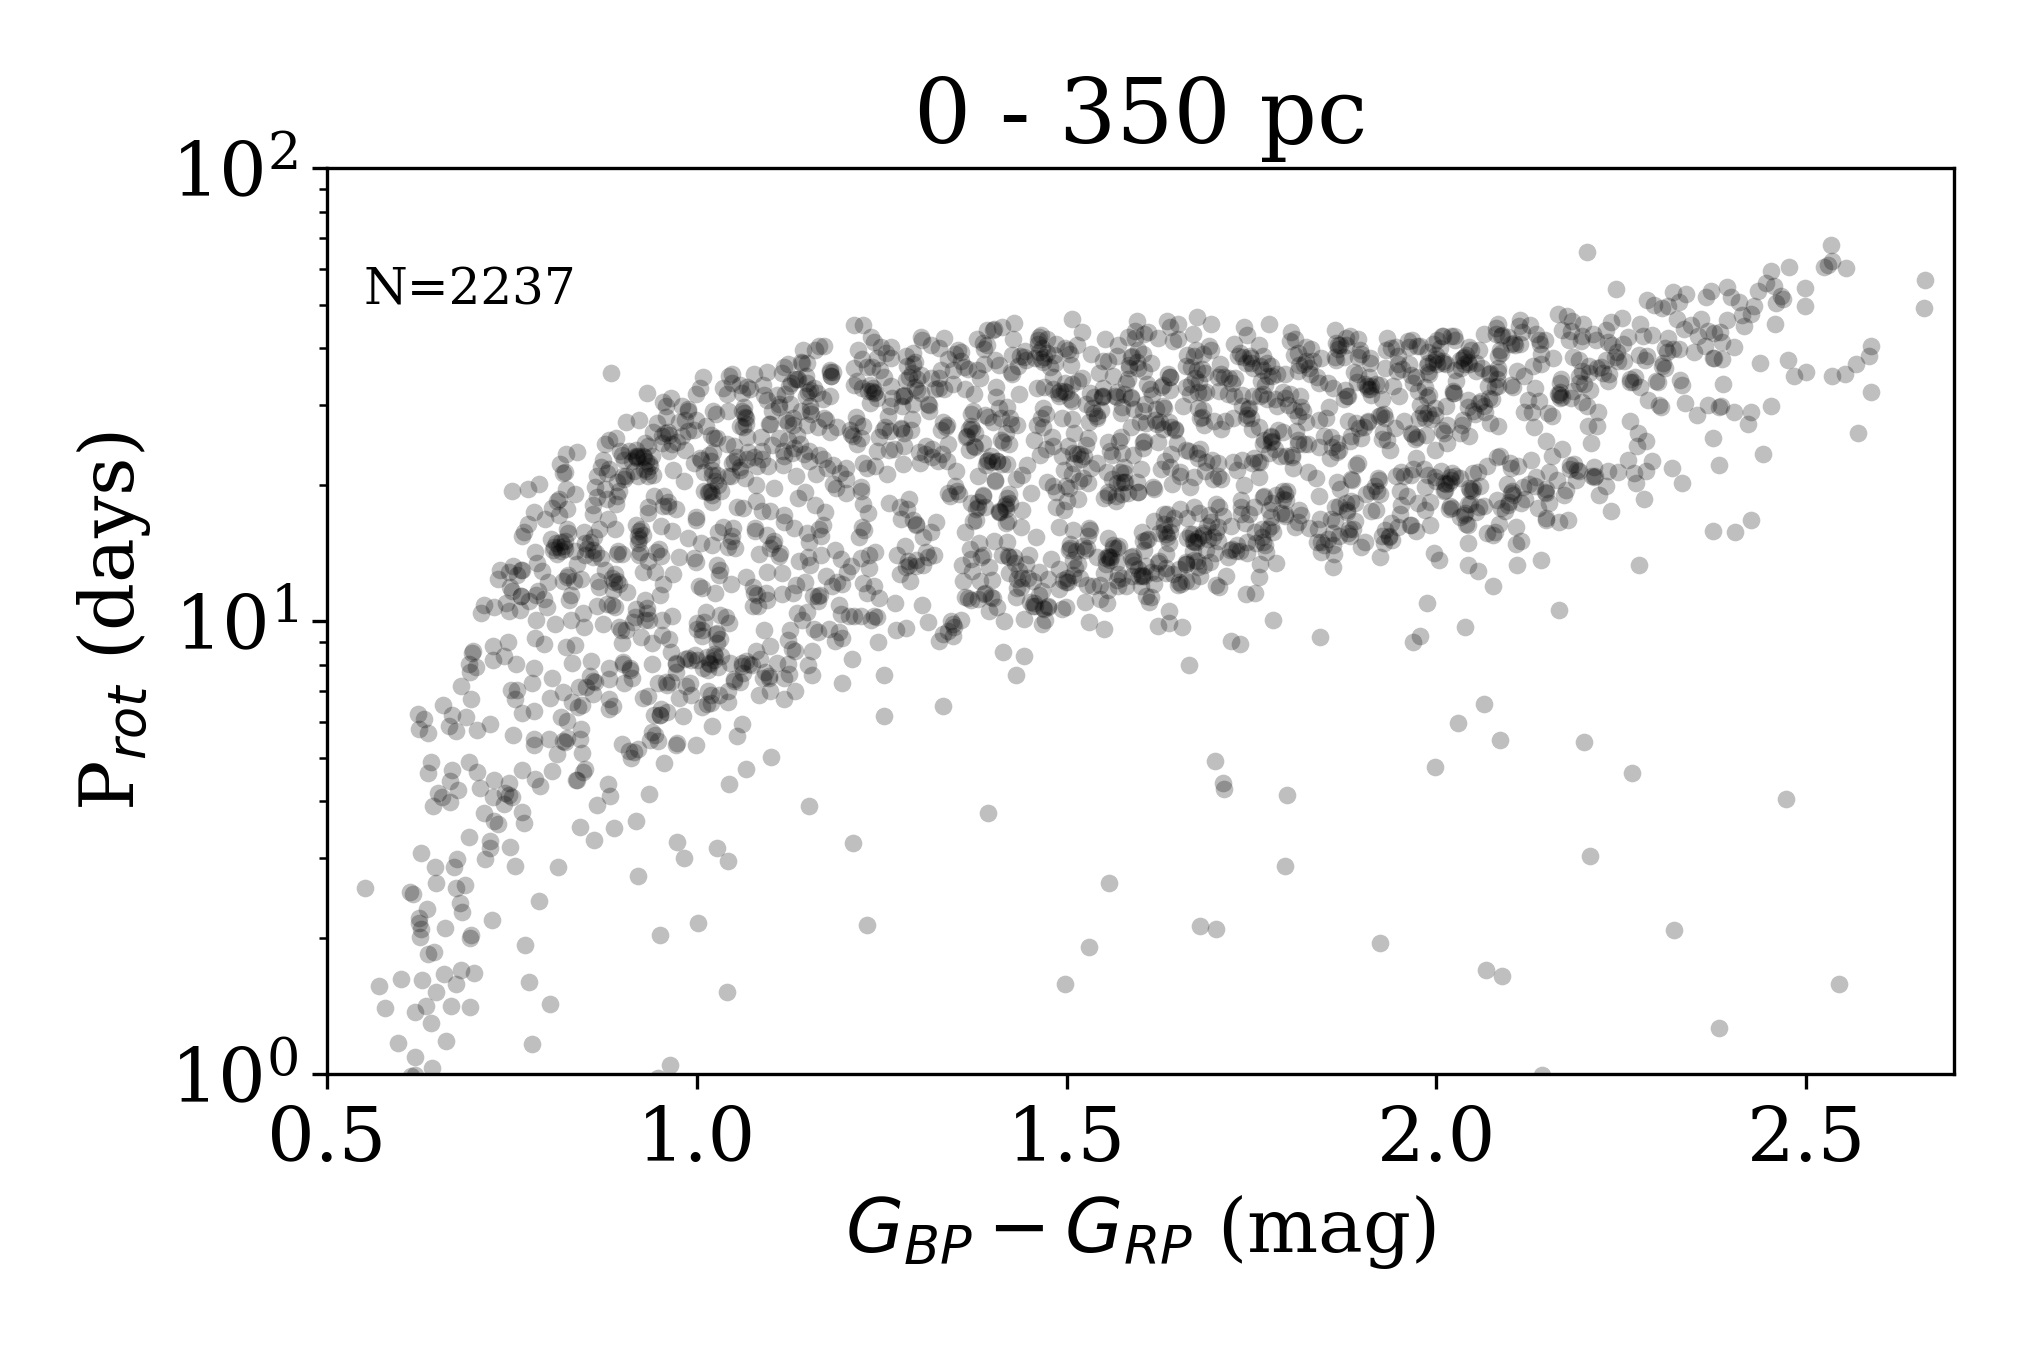
\includegraphics[width=3.5in]{../figures/rot_dist_0}
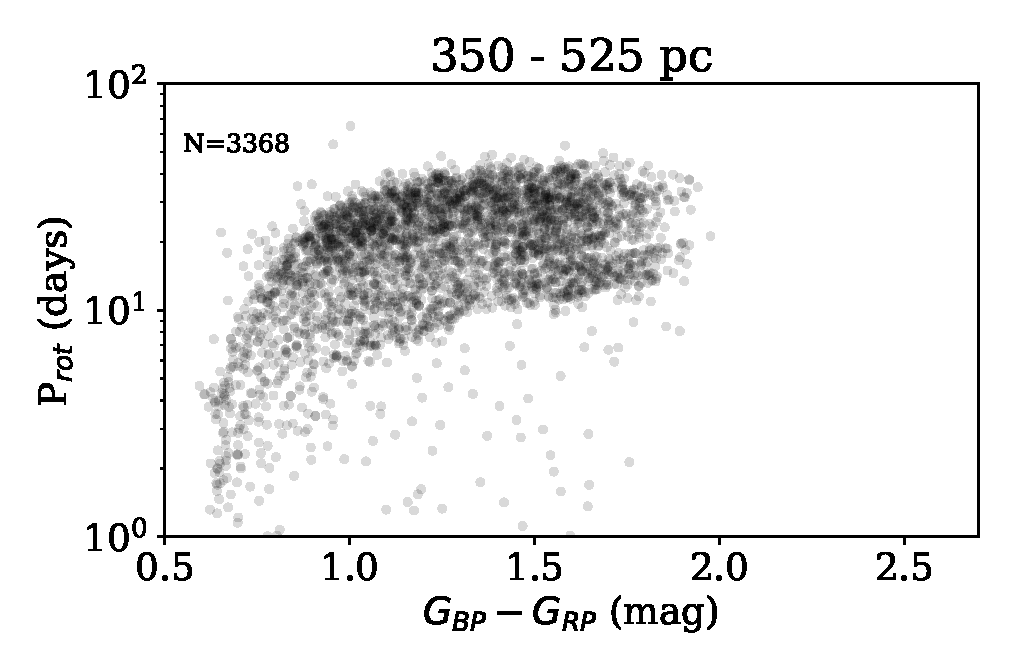
\includegraphics[width=3.5in]{../figures/rot_dist_350}
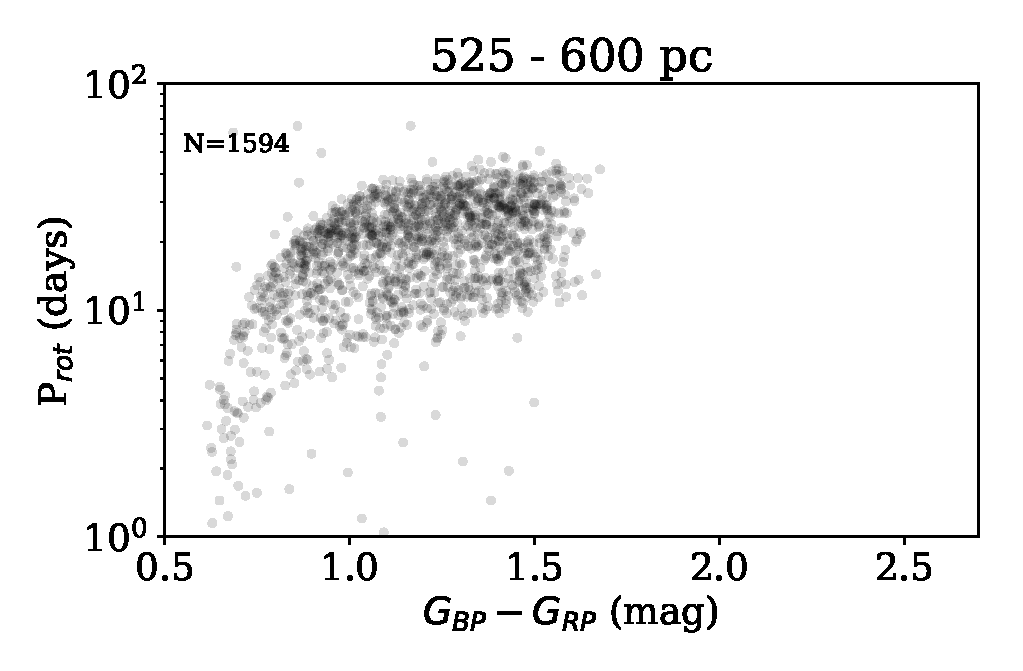
\includegraphics[width=3.5in]{../figures/rot_dist_525}
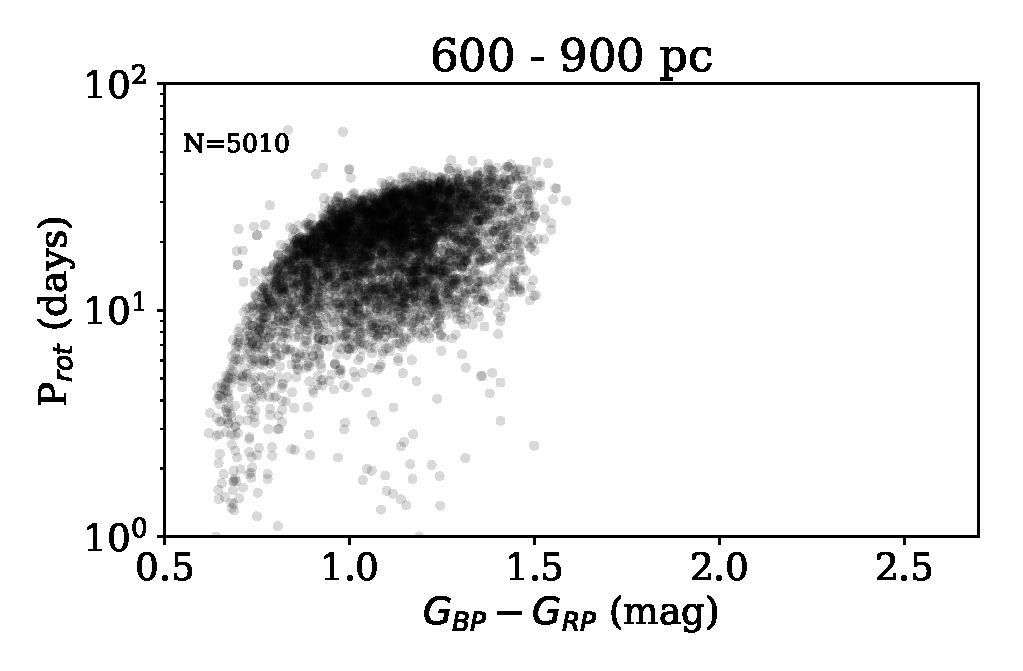
\includegraphics[width=3.5in]{../figures/rot_dist_600}
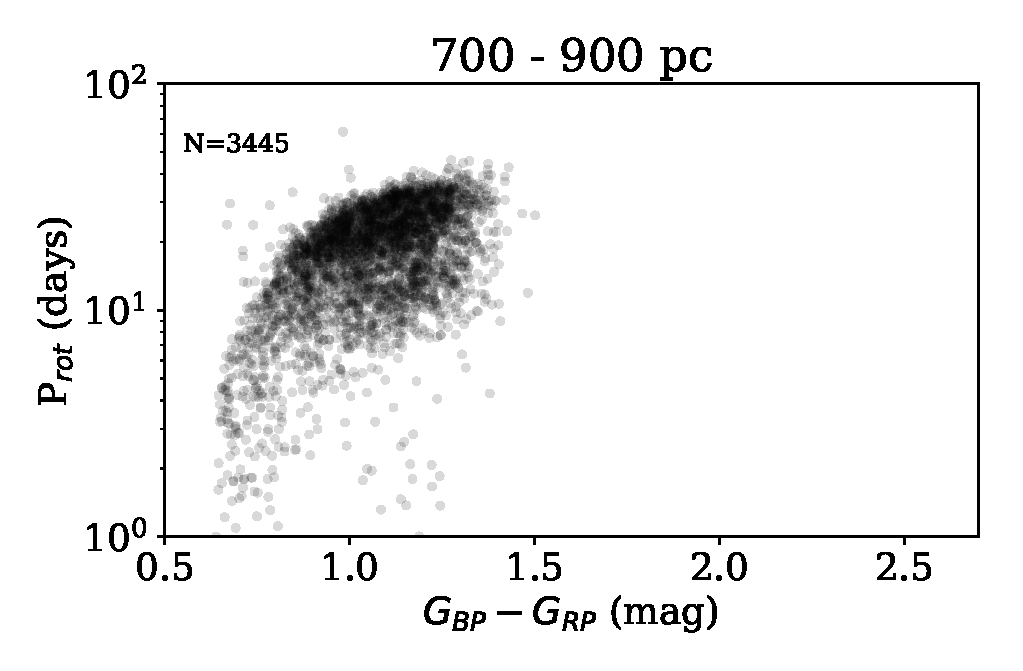
\includegraphics[width=3.5in]{../figures/rot_dist_700}
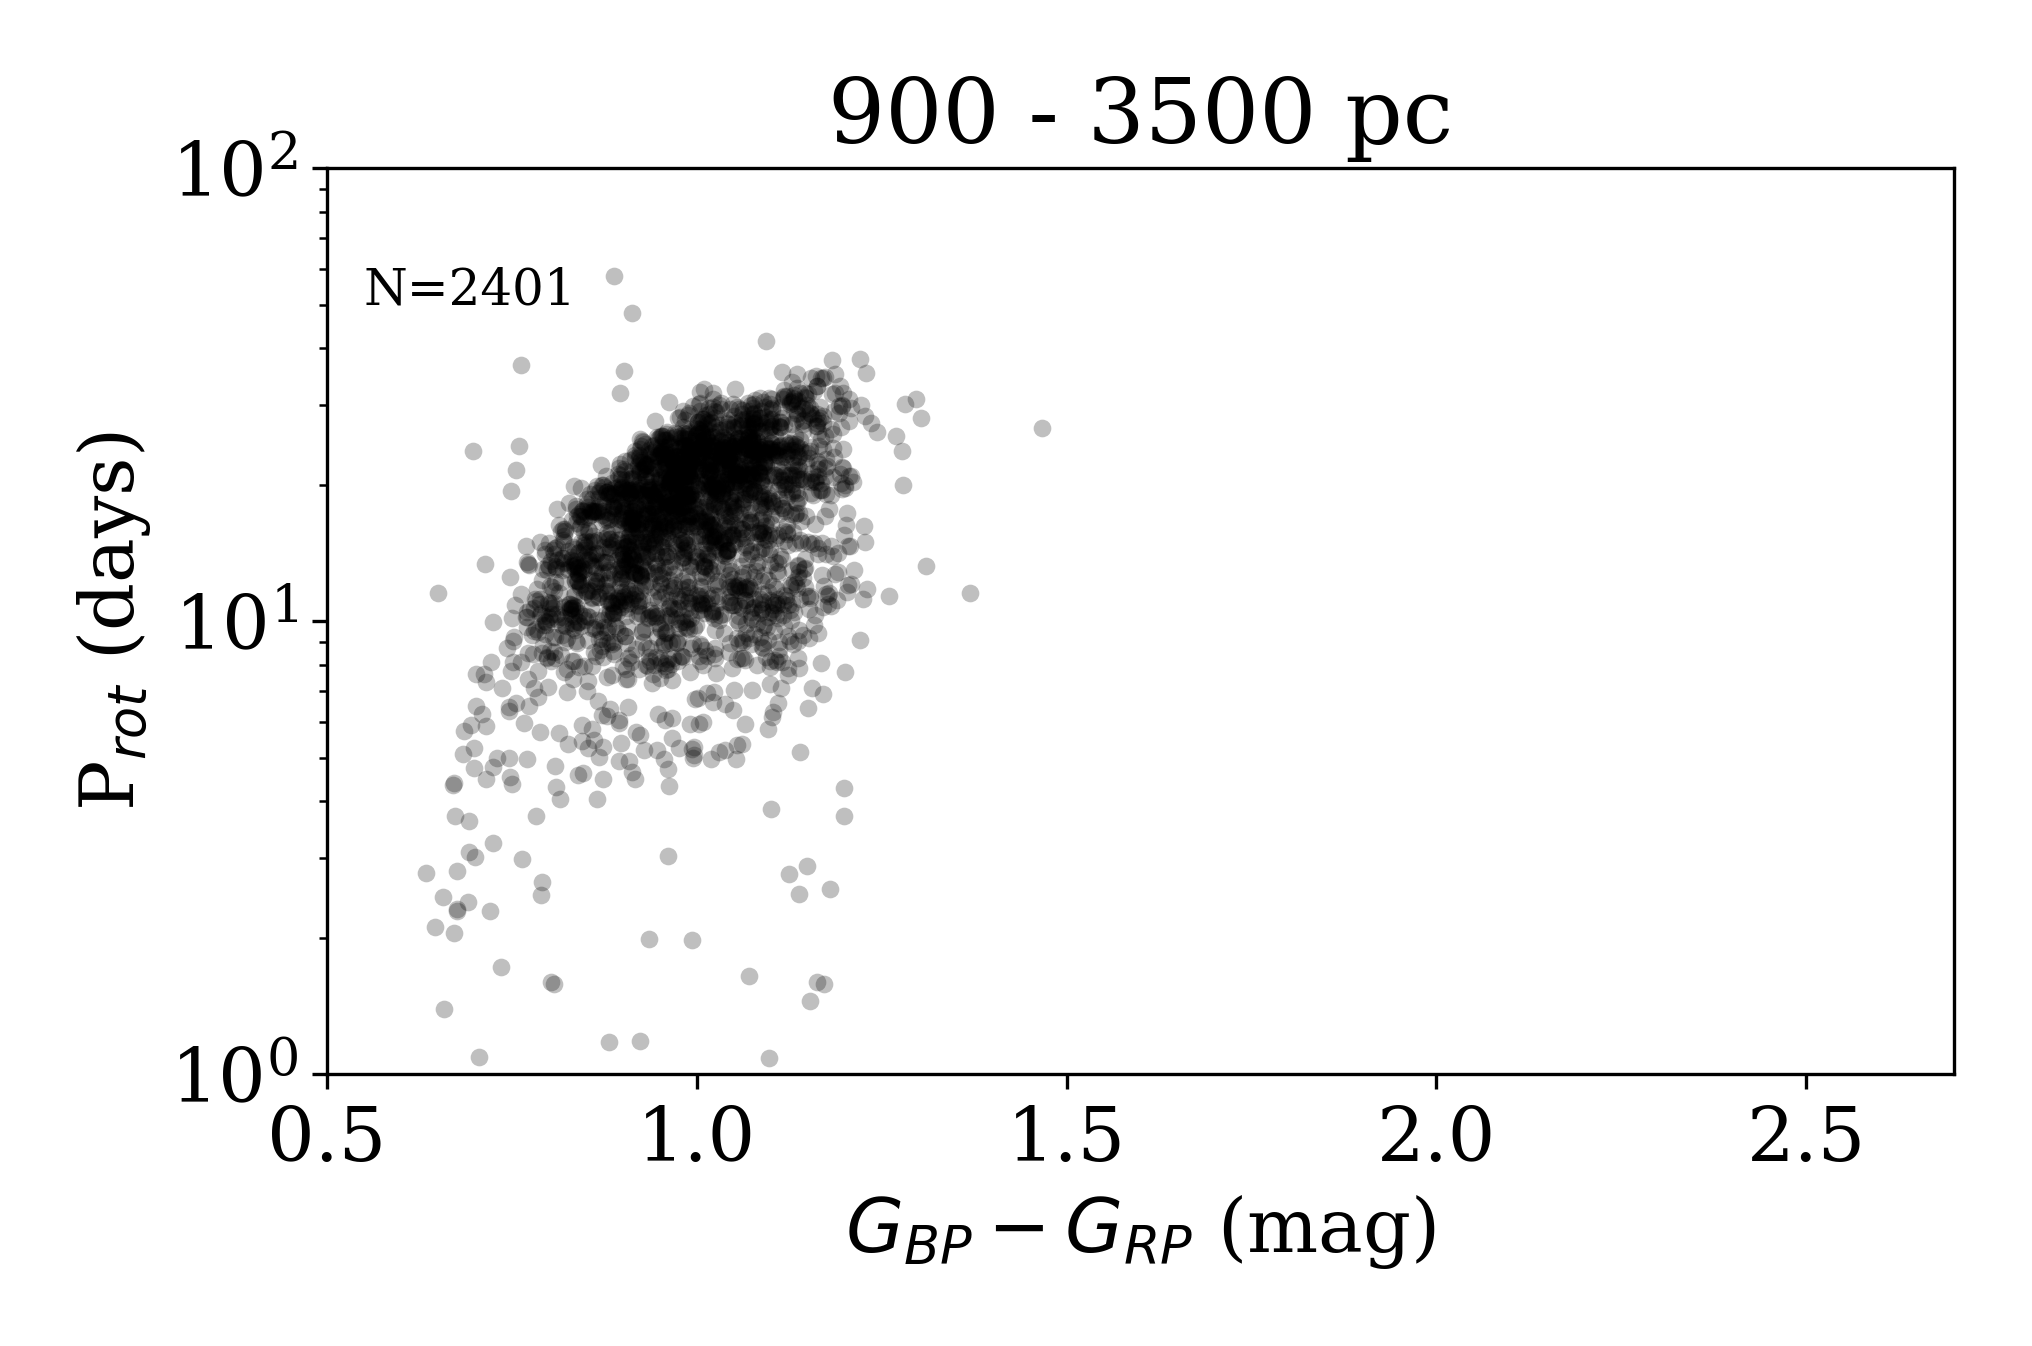
\includegraphics[width=3.5in]{../figures/rot_dist_900}
\caption{Color--period diagrams for our sample of likely main sequence stars, divided into six bins of distance. Our nearest bin (within 350pc) is effectively the distance analyzed in \citet{davenport2017} using Gaia DR1, and clearly shows the rotation period bimodality for the entire sample. The brighter magnitude limit of the \Kepler sample results in redder (fainter) stars missing in our further distance bins. The rotation period bimodality can be seen in the 350-525 pc bin, but is not found in the bluer stars at further distances.
}
\label{fig:color_period}
\end{figure*}

Using this sample of likely single, main sequence stars from \Kepler and {\em Gaia}, we are able to explore the distribution of rotation periods for stars as a function of their distance. The rotation period bimodality in \Kepler stars previously only detected for stars within $\sim$300 pc of the Sun due to the limits of available parallax data. Now with {\em Gaia} DR2, our sample of main sequence star with measured rotation periods in \Kepler extends out to over 2 kpc.

In Figure \ref{fig:color_period} we present the period--color diagram for our sample of stars, split into six bins of projected distance. The first panel (0--350 pc) effectively reproduces the results of \citet{davenport2017} for bluer stars and \citet{mcquillan2014} for the redder stars. A gap in the observed rotation periods as a function of color is seen, at a period of approximately 5 days for $G_{BP}-G_{RP}\approx1$, 20 days for $G_{BP}-G_{RP}\approx2$, and increasing towards 30 days for the reddest stars in our sample. This gap corresponds with a line of approximately constant age, consistent with a gyrochrone with age $\sim$600 Myr \citep{davenport2017}. 



The bimodality is still apparent in the second distance bin (350--525 pc), clearly visible in the redder stars, but seems to fade in the final three bins. Other structures in the period distributions are visible, however. For example, a thin sequence of stars with rotation periods near 10 days is faintly visible in the most distant bin (900--2500 pc) for stars with colors of $0.8<G_{BP}-G_{RP}<1.2$. This feature is due to the 1 Gyr open cluster NGC 6811 in the \Kepler field \citep{meibom2011}, whose distance is $\sim$1100 pc \citep{sandquist2016}.



\begin{figure*}[!t]
\centering
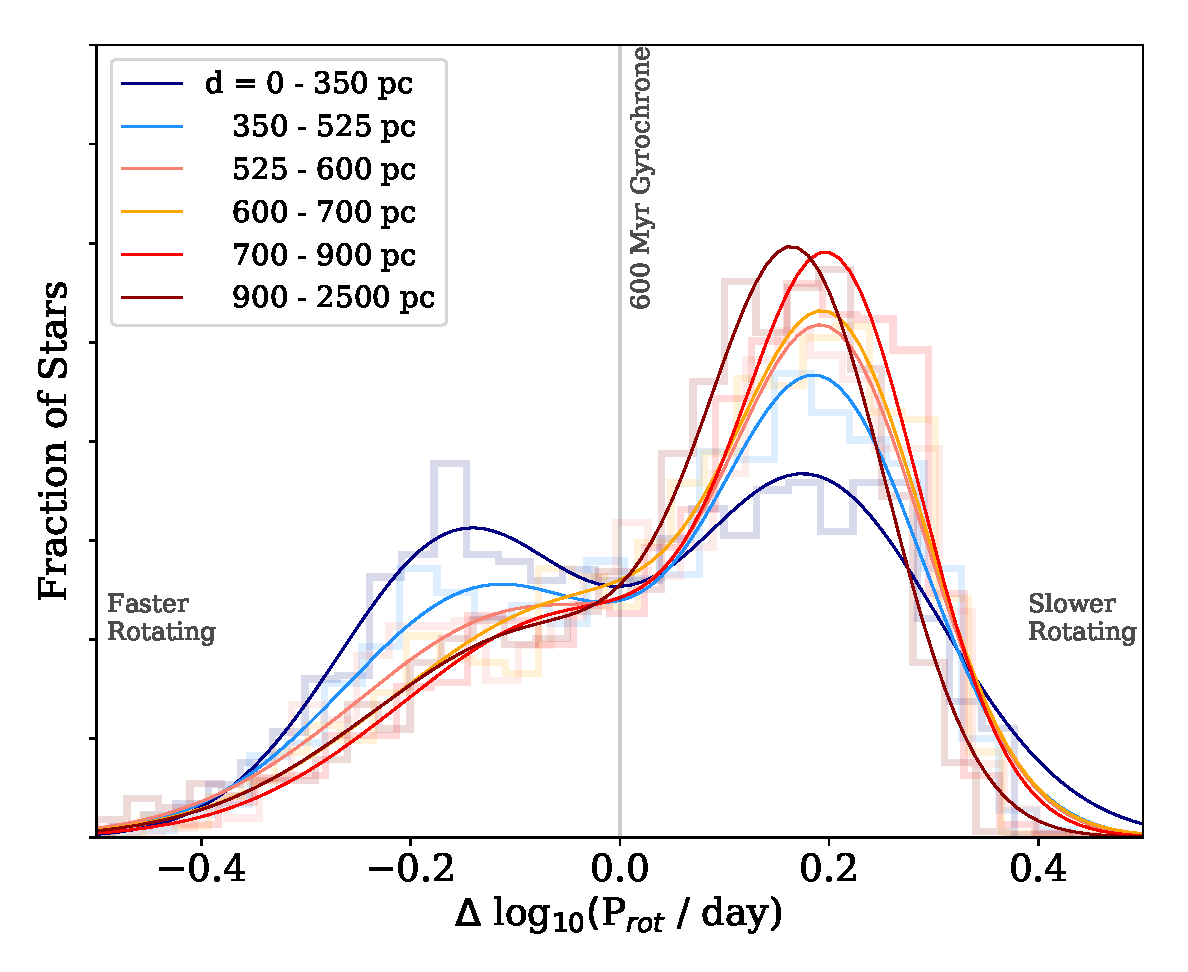
\includegraphics[width=3.5in]{../figures/delta_per_2gauss}
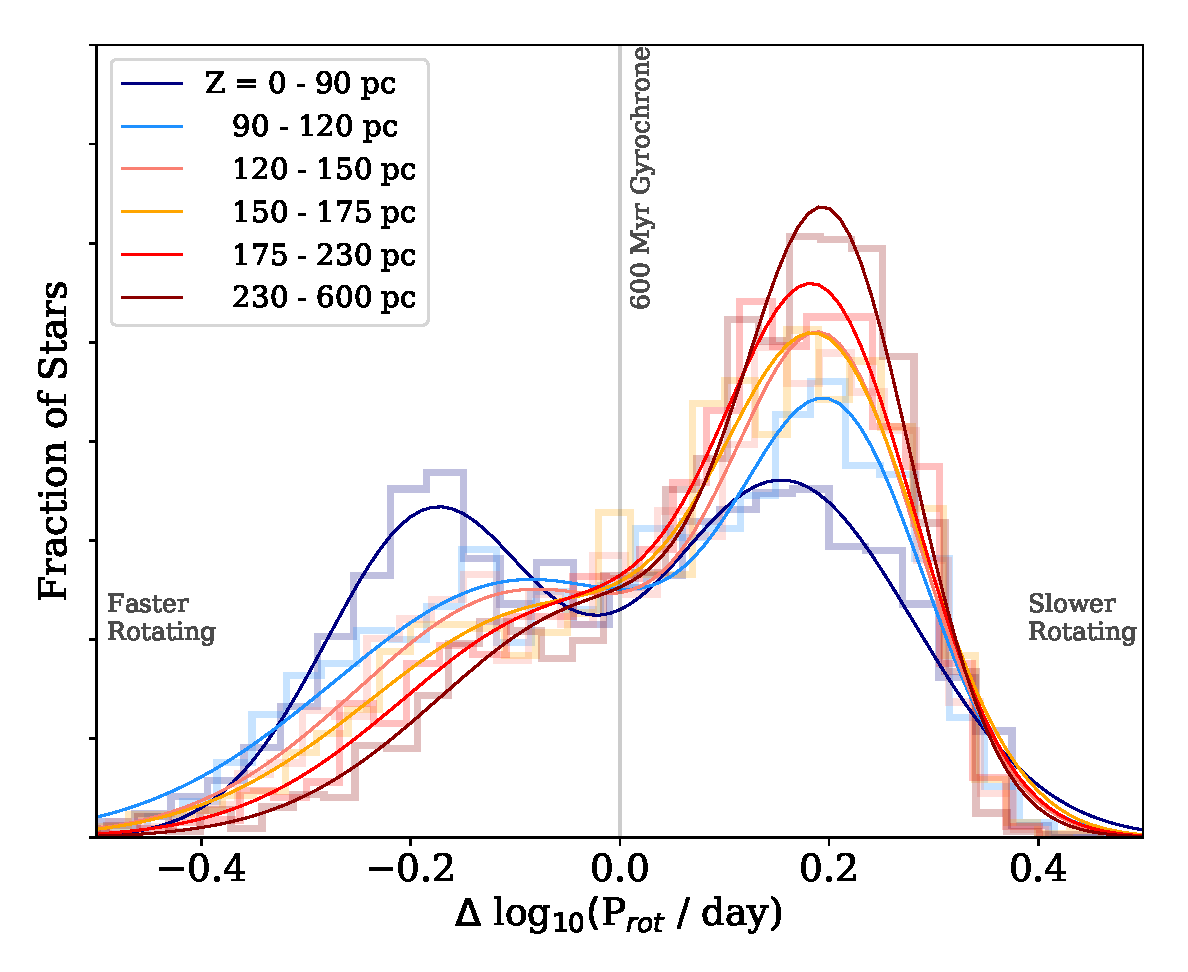
\includegraphics[width=3.5in]{../figures/delta_per_2gauss_Z}
\caption{Left: Distribution of the log rotation periods after a 600 Myr gyrochrone was subtracted, using the same distance bins shown in Figure \ref{fig:color_period} (faint lines). Two-gaussian models were fit to each histogram (bold lines). 
The rotation period bimodality for stars within 350 pc has two nearly equal peaks similar to those found in \citet{davenport2017}, at -0.15 and +0.18 dex. The fast rotating peak (left side) declines sharply at further distances.
Right: Same as Left, but in bins of Galactic height above the plane (Z). The drop-off of fast rotating, young stars is even more pronounced as a function of height.
}
\label{fig:per_hist}
\end{figure*}


To better illustrate the evolution of rotation periods for all the stars between the distance bins, in Figure \ref{fig:per_hist} we follow \citet{davenport2017} and subtract the rotation period of a 600 Myr gyrochrone. As no published gyrochronology model yet exists that has been tuned to the {\em Gaia} photometric colors, we adopt the same gyrochronology model of Eqn. 2 from \citet{meibom2009} used by \citet{davenport2017} to approximately trace the rotation period gap at 600 Myr as a function of $B-V$ color. We convert stars from the observed {\em Gaia} $G_{BP}-G_{RP}$ color to $B-V$ using the same 1 Gyr MIST isochrone model used to define the main sequence in Figure \ref{fig:cmd} above. 

Our sample naturally becomes biased towards the bluer (brighter) stars as we reach larger distances. Since bluer stars have more rapid rotation and more dramatic period evolution, gyrochronology models are ``bent'' strongly for these stars, and thus the period bimodality (or other structures) become difficult to distinguish. \citet{davenport2017} used an ad-hoc modification of the gyrochrone model for the hottest stars to illustrate the existence of the period bimodality. However, in Figure \ref{fig:per_hist} we limit our analysis to stars with $0.8<B-V<1.5$ (approximately $0.9<G_{BP}-G_{RP}<2.2$, or $0.9>M_\odot> 0.5$), where the gyrochrone is most flat as a function of color. This color range was chosen to ensure ample stars were available in each distance bin, but without having to use the ad-hoc gyrochrone model correction from \citet{davenport2017}.



Figure \ref{fig:per_hist} (left) shows clearly that for the short period component of the rotation period bimodality dominates only for the nearest stars, and steadily decreases with increasing distance.
%but can also cut vs Z instead of d. See bimodality drops neatly with height in Figure \ref{fig:per_hist} also.
The \Kepler field is centered on a Galactic latitude of $b\sim13.5^\circ$, and so we can also study the period bimodality as a function of height above the Galactic mid-plane.
Both galaxy formation simulations \citep{ma2017} and observations of stars in the nearby Milky Way \citep{xiang2017} indicate that height above the mid-plane correlates strongly with the median ages for stars, out to distances of several kpc. The Milky Way thin disk has a scaleheight of $\sim$300 pc \citep{gilmore1983}.
However, since the \Kepler field is oriented towards low latitudes we do not reach significant {\it heights} above the disk.
The projected height above the mid-plane for the distance bins shown in Figures \ref{fig:color_period} and \ref{fig:per_hist} ranges from $Z\sim100$ pc at a distance of $d=350$ pc to $Z\sim230$ pc at $d=900$ pc. As a result, we are only sensitive to changes in the youngest stars within this span of $Z$.

In Figure \ref{fig:per_hist} (right) we find that the drop-off of the short-period (rapid rotating) component of the period bimodality is even more pronounced as a function of $Z$, decreasing rapidly after only 90 pc. With increasing height we also see that the shift to the longer period component is more smooth. However, from these two projections in Figure \ref{fig:per_hist} alone (distance and height) we cannot definitively determine the spatial structure of the rotation period bimodality.


As a first attempt at understanding the spatial extent of this age-related feature, in Figure \ref{fig:dZ} we break the lowest height stars ($Z < 100$ pc) in to two roughly even samples, split as a function of their projected distance. Note we have also repeated this exercise for stars in higher ranges of $Z$, and find the decline of the rapid rotators is again uniform between subsamples of varying projected distance. The rotation period bimodality is clearly seen in both distance bins of Figure \ref{fig:dZ}, indicating that the feature is likely not a localized star formation history artifact centered around the Sun. Instead, we believe this feature is characteristic of the age--$Z$ dynamical correlation observed within the solar neighborhood of our Galaxy. 


\begin{figure}[!ht]
\centering
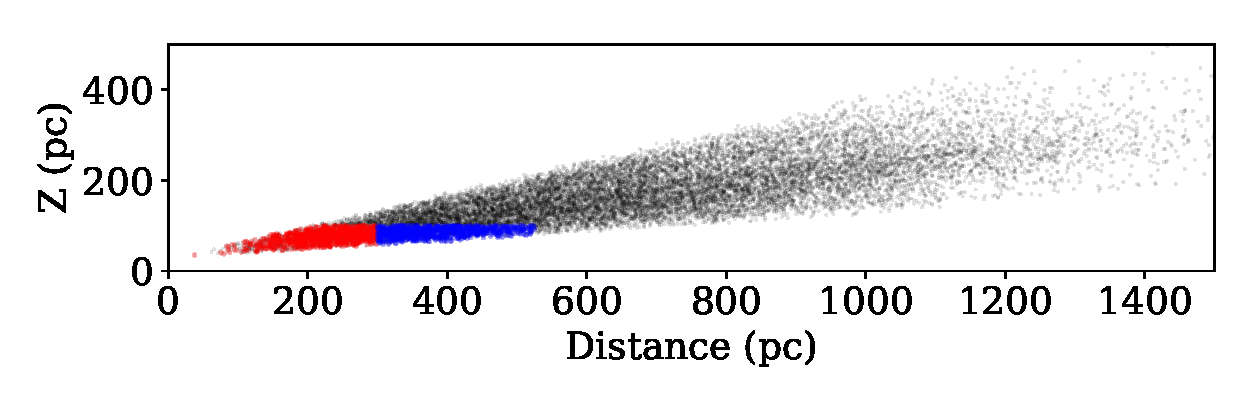
\includegraphics[width=3.3in]{../figures/dist_Z}
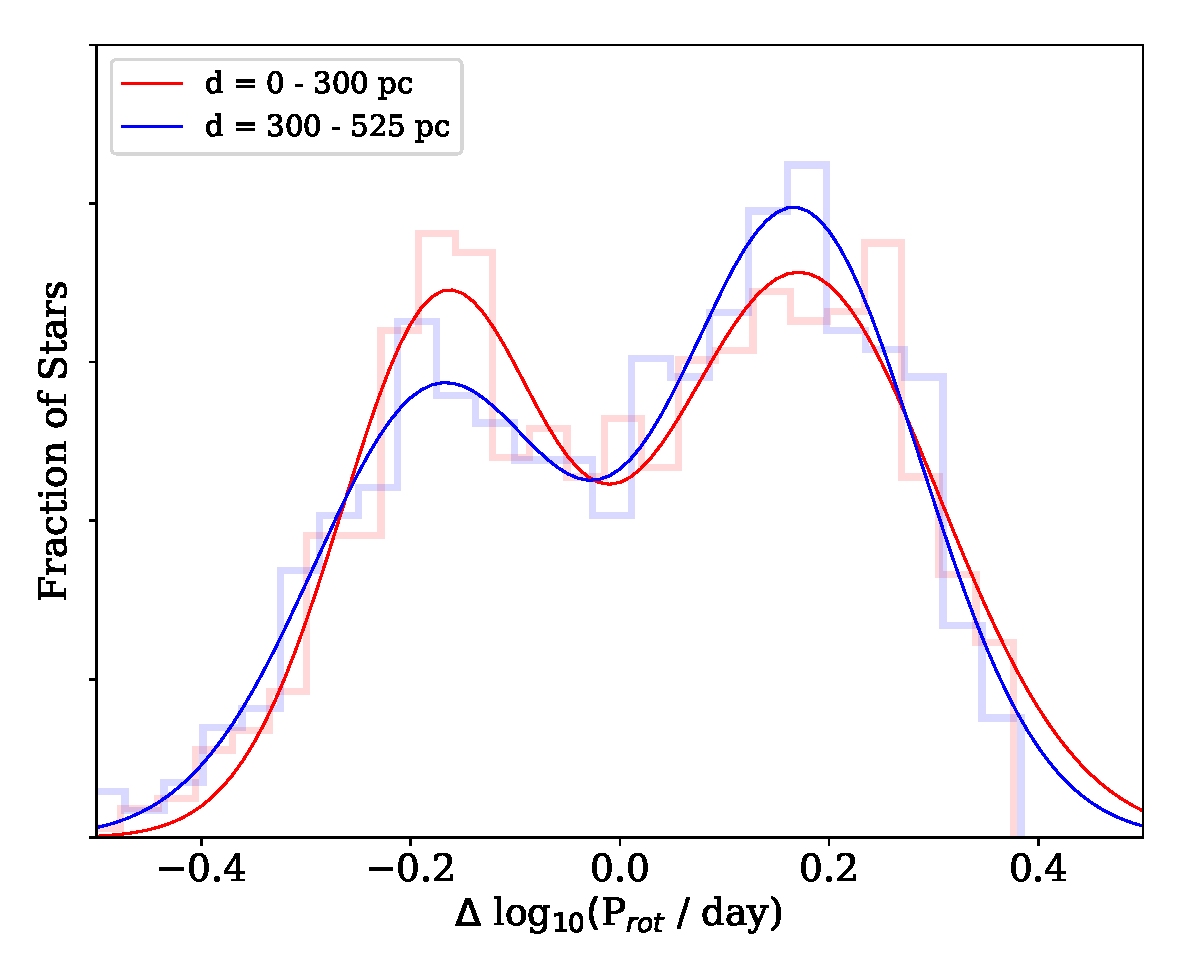
\includegraphics[width=3.5in]{../figures/delta_per_subZ}
\caption{
Top: projected distance and Galactic height of the main sequence stars in our sample. Two approximately equal subsets of stars near the Galactic mid-plane have been highlighted, those with distances from the sun of $d<300$ pc (red), and with $300<d<525$ pc.
Bottom: As in Figure \ref{fig:per_hist}, the distribution of rotation periods after a 600 Myr gyrochrone was subtracted (faint lines), and with two-Gaussian fits (bold lines) for the same subsets of stars as above. The period bidmodality is seen in both distance bins, suggesting it is not localized around the Sun.
}
\label{fig:dZ}
\end{figure}




%%%%%%%%%%%%%%%%%%%%%%
\section{Recalibrating Stellar Evolution Models}


\begin{figure*}
\centering
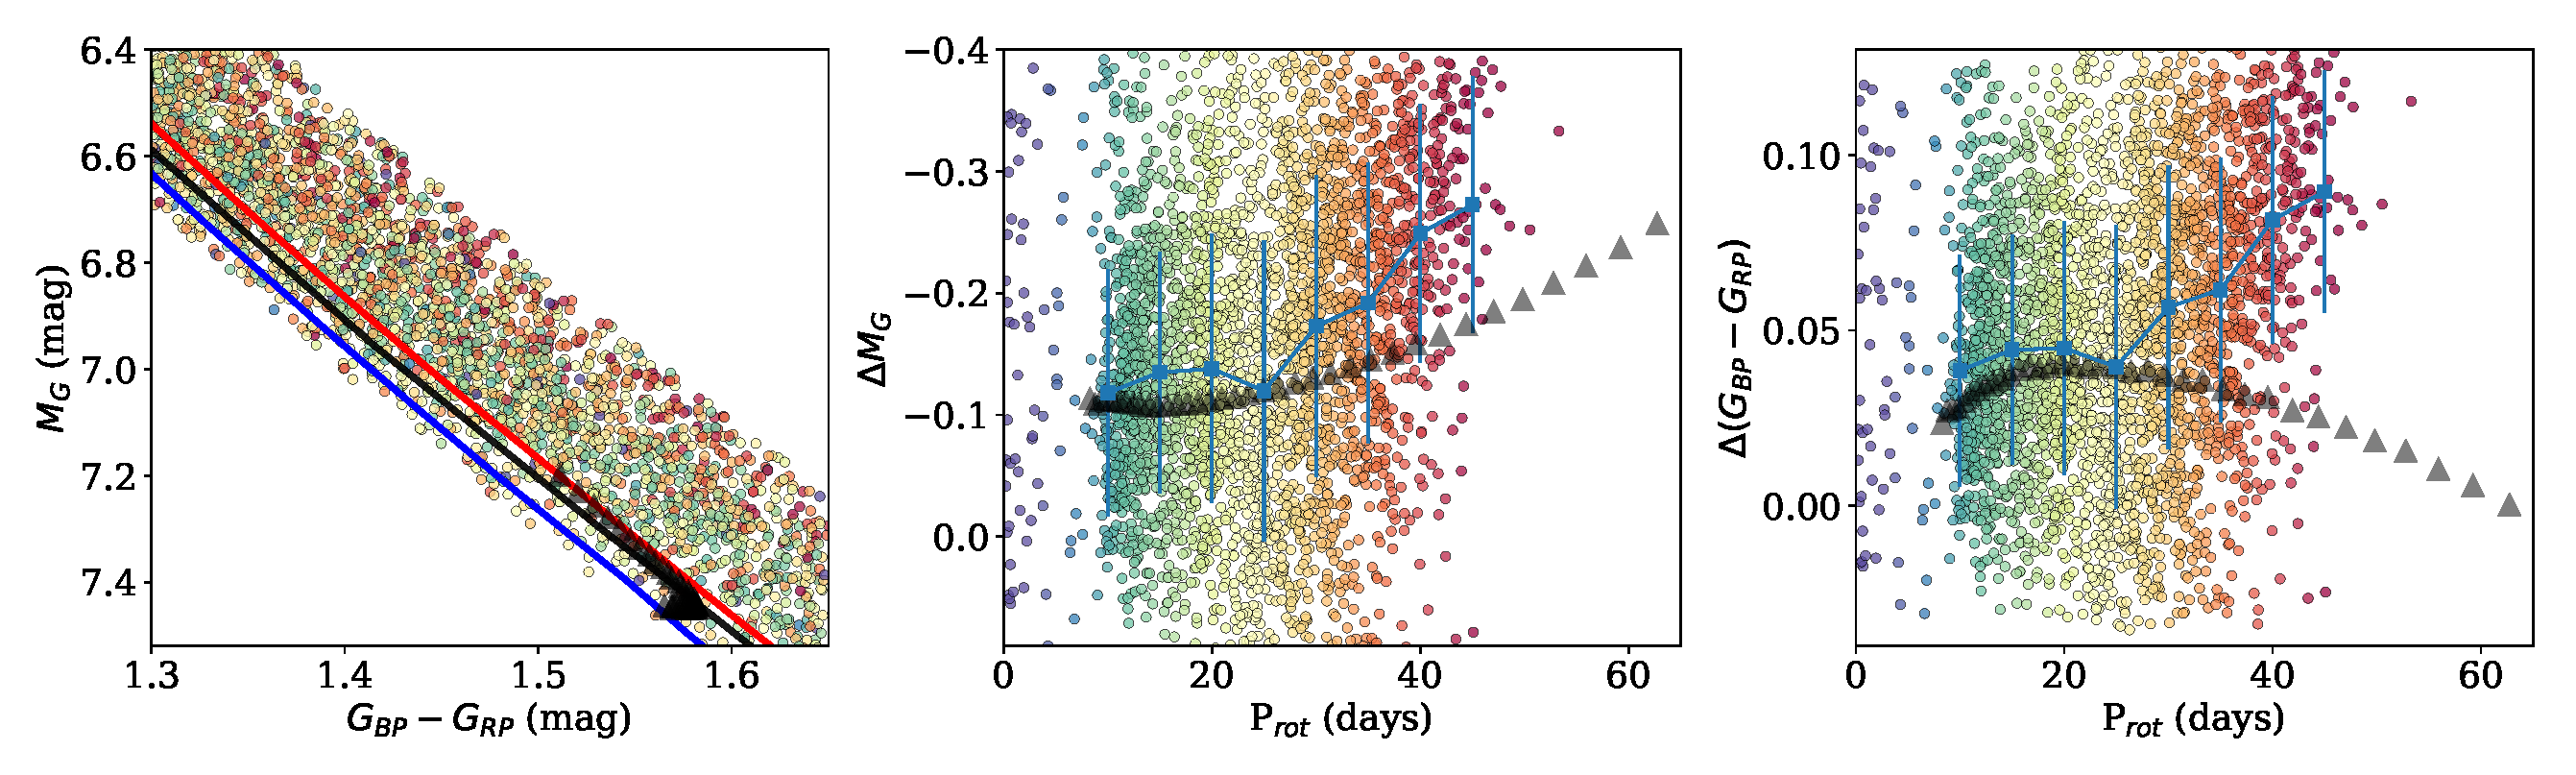
\includegraphics[width=6in]{../figures/cmd_zoom}
\caption{
Left: Enlarged portion of the color--magnitude diagram from Figure \ref{fig:cmd} in a region centered near $\sim$0.75 M$_\odot$, with stars are colored by their measured \Kepler rotation periods from \citet{mcquillan2014}.
MIST isochrones at ages of $10^8$, $10^9$, and $10^{10}$ yr are shown for comparison (blue, black, and red lines). The predicted evolution of a 0.7 M$_\odot$ star is highlighted (black triangles). 
Right: Difference in $M_G$ from the $10^9$ yr MIST isochrone as a function of rotation period (point color again indicates rotation period, as in Left panel). Blue squares show an increase in the median $M_G$ offset in bins of increasing rotation period. Error bars shown are the standard deviation of $\Delta M_G$ in each bin. The 0.7 M$_\odot$ star brightness evolution is shown as a function of rotation evolution from \citet{meibom2009} (black triangles).
}
\label{fig:cmd_zoom}
\end{figure*}

A subtle feature we noticed in Figure \ref{fig:cmd} is the color gradient (i.e. rotation period gradient) for the stars in between the single and binary star main sequence populations. In Figure \ref{fig:cmd} this appears as a yellow stripe (i.e. rotation periods of 30-40 days) between these blue-green sequences for systems with colors of $G_{BP} - G_{RP} \approx 1.5$. To exaggerate this feature, we have reproduced a portion of our color--magnitude diagram focused on the main sequence near this stellar color in the left panel of Figure \ref{fig:cmd_zoom}. A clear color gradient is present, with red points (slower rotators) appearing preferentially above the main sequence.
The right panel of Figure \ref{fig:cmd_zoom} concretely demonstrates a correlation between the measured rotation period and the vertical offset (i.e. absolute magnitude) from the $10^9$ year MIST isochrone. Slower rotating stars are brighter at a given color.

We interpret this observation as being due to the increase in luminosity of stars across their main sequence lives, coupled with the angular momentum loss that underpins gyrochronology. Indeed, the three MIST isochrones shown in Figure \ref{fig:cmd_zoom} with ages of $10^8$, $10^9$, and $10^{10}$ years clearly predicts a net increase in brightness of the main sequence over time. We also track the color--magnitude evolution of a 0.7 $M_\odot$ star over its lifetime in Figure \ref{fig:cmd_zoom}, which shows the ``hook'' the star takes over its main sequence life. 

Inverting the color--magnitude diagram into precise ages for main sequence stars using {\em Gaia} is beyond scope of this work. However, Figure \ref{fig:cmd_zoom} clearly demonstrates that age information is not only present in the CMD for main sequence stars, but it may also be a larger amplitude effect than previously assumed. For example: younger, presumably more metal rich stars, should have redder main sequence colors. This in turn should move the entire main sequence track to the right in the CMD. However, we find older stars (slower rotators) appearing on the right side of the main sequence, due to their increased luminosity with age. The main sequence location of a star is therefore not simply due to its mass and metallicity in the {\em Gaia} era, but its age must also be taken into account.

In Figure \ref{fig:cmd_zoom} we also show the change in brightness as a function of the rotation period for the stars in our zoomed-in CMD, as well as a prediction for the evolution of a 0.7 $M_\odot$ star. The spin-down model here is a combination of the MIST isochrone evolution, as well as the \citet{meibom2009} gyrochronology model. Note this spin-down model has been arbitrarily offset in the $\Delta M_G$ to roughly go through the observed data at the rapid rotation end.
While \Kepler light curves generally are not able to measure rotation periods reliably with periods longer than 20 or 30 days, we find that stars with brightness (vertical) offsets in the CMD consistent with being several Gyr old have average rotation periods far shorter than the 60--80 days values predicted from the spin-down models.

One interpretation of this result may be that the older stars are spinning {\it faster} than expected for stars their age. This is qualitatively similar to the model of broken spin-down occurring at a critical Rossby number suggested by \citet{van-saders2016}. Though we cannot definitively confirm such intriguing rotation evolution from this initial investigation given the observation bias for long periods from \Kepler, matching the {\em Gaia} CMD with other rotation period measurements may provide an ideal dataset to test the \citet{van-saders2016} model against. The ability to simultaneously constrain the precise CMD location and surface rotation rate, as with the sample demonstrated here, may also be a valuable method for calibrating a new generation of isochrone and gyrochronology models.





%%%%%%%%%%%%%%%%%%%%%%
\section{Discussion}
%% HERE

% from paper1
%
%The period bimodality may yet be a manifestation of the ``Vaughan-Preston'' gap observed in chromospheric activity indicators from solar type stars. Such a feature has also been discussed for rotating stars by \citet{kado-fong2016}. Given that the mass range for the bimodality explored 

we find period bimodality is localized to low galactic heights, not only close distances to the Sun.
using rotation to trace the ages of nearby stars. would be really neat to compare the spatial structure of star formation in detail, as 
\citet{lewis2015} for example show lots of variation in SFH in 100pc bins for M31
%\citet{williams2017} also for M31, older SFH tracers
and find out what the actual extent/coherance of the bimodality is. 

Adding to the sample of rotation periods from Kepler using K2 (Foreman-Mackey in prep?), not only for doubling the sample size to investigate trends with more precision, but also the wider range of galactic fields of view mean wider range of ages/SFH's we can sample. 

We note a shortcoming of our approach in normalizing the rotation period distributions to a 600 Myr gyrochrone in Figure \ref{fig:per_hist} is that it gives the false appearance that this age is a universal transition point. A more robust approach is needed that uses improved gyrochronology models to invert the observed color--period diagrams into age distributions. 


finally, this work has found strong motivation for a new generation of gyrochronology isochrones to adequately model the {\em Gaia}--\Kepler/K2 (and soon TESS) rotation data for field stars. As we show in Figure \ref{fig:cmd_zoom}, these models should include both the angular momentum evolution (period), as well as the temperature and luminosity (color, magnitude) as a function of time. With such improvements, we may be able to 



%%%%%%%%%%%%%%%%%
\acknowledgments

JRAD is supported by an NSF Astronomy and Astrophysics Postdoctoral Fellowship under award AST-1501418. 

This work made use of the \url{gaia-kepler.fun} crossmatch database, created by Megan Bedell.

This project was developed in part at the 2018 Gaia Sprint, hosted by the eScience and DIRAC Institutes at the University of Washington, Seattle, in parallel with the 2018 NYC Gaia Sprint, hosted by the Center for Computational Astrophysics at the Simons Foundation in New York City.

This work has made use of data from the European Space Agency (ESA) mission
{\it Gaia} (\url{https://www.cosmos.esa.int/gaia}), processed by the {\it Gaia}
Data Processing and Analysis Consortium (DPAC,
\url{https://www.cosmos.esa.int/web/gaia/dpac/consortium}). Funding for the DPAC
has been provided by national institutions, in particular the institutions
participating in the {\it Gaia} Multilateral Agreement.



\bibliography{/Users/james/Dropbox/references}

\end{document}
